\documentclass[1p]{elsarticle_modified}
%\bibliographystyle{elsarticle-num}

%\usepackage[colorlinks]{hyperref}
%\usepackage{abbrmath_seonhwa} %\Abb, \Ascr, \Acal ,\Abf, \Afrak
\usepackage{amsfonts}
\usepackage{amssymb}
\usepackage{amsmath}
\usepackage{amsthm}
\usepackage{scalefnt}
\usepackage{amsbsy}
\usepackage{kotex}
\usepackage{caption}
\usepackage{subfig}
\usepackage{color}
\usepackage{graphicx}
\usepackage{xcolor} %% white, black, red, green, blue, cyan, magenta, yellow
\usepackage{float}
\usepackage{setspace}
\usepackage{hyperref}

\usepackage{tikz}
\usetikzlibrary{arrows}

\usepackage{multirow}
\usepackage{array} % fixed length table
\usepackage{hhline}

%%%%%%%%%%%%%%%%%%%%%
\makeatletter
\renewcommand*\env@matrix[1][\arraystretch]{%
	\edef\arraystretch{#1}%
	\hskip -\arraycolsep
	\let\@ifnextchar\new@ifnextchar
	\array{*\c@MaxMatrixCols c}}
\makeatother %https://tex.stackexchange.com/questions/14071/how-can-i-increase-the-line-spacing-in-a-matrix
%%%%%%%%%%%%%%%

\usepackage[normalem]{ulem}

\newcommand{\msout}[1]{\ifmmode\text{\sout{\ensuremath{#1}}}\else\sout{#1}\fi}
%SOURCE: \msout is \stkout macro in https://tex.stackexchange.com/questions/20609/strikeout-in-math-mode

\newcommand{\cancel}[1]{
	\ifmmode
	{\color{red}\msout{#1}}
	\else
	{\color{red}\sout{#1}}
	\fi
}

\newcommand{\add}[1]{
	{\color{blue}\uwave{#1}}
}

\newcommand{\replace}[2]{
	\ifmmode
	{\color{red}\msout{#1}}{\color{blue}\uwave{#2}}
	\else
	{\color{red}\sout{#1}}{\color{blue}\uwave{#2}}
	\fi
}

\newcommand{\Sol}{\mathcal{S}} %segment
\newcommand{\D}{D} %diagram
\newcommand{\A}{\mathcal{A}} %arc


%%%%%%%%%%%%%%%%%%%%%%%%%%%%%5 test

\def\sl{\operatorname{\textup{SL}}(2,\Cbb)}
\def\psl{\operatorname{\textup{PSL}}(2,\Cbb)}
\def\quan{\mkern 1mu \triangleright \mkern 1mu}

\theoremstyle{definition}
\newtheorem{thm}{Theorem}[section]
\newtheorem{prop}[thm]{Proposition}
\newtheorem{lem}[thm]{Lemma}
\newtheorem{ques}[thm]{Question}
\newtheorem{cor}[thm]{Corollary}
\newtheorem{defn}[thm]{Definition}
\newtheorem{exam}[thm]{Example}
\newtheorem{rmk}[thm]{Remark}
\newtheorem{alg}[thm]{Algorithm}

\newcommand{\I}{\sqrt{-1}}
\begin{document}

%\begin{frontmatter}
%
%\title{Boundary parabolic representations of knots up to 8 crossings}
%
%%% Group authors per affiliation:
%\author{Yunhi Cho} 
%\address{Department of Mathematics, University of Seoul, Seoul, Korea}
%\ead{yhcho@uos.ac.kr}
%
%
%\author{Seonhwa Kim} %\fnref{s_kim}}
%\address{Center for Geometry and Physics, Institute for Basic Science, Pohang, 37673, Korea}
%\ead{ryeona17@ibs.re.kr}
%
%\author{Hyuk Kim}
%\address{Department of Mathematical Sciences, Seoul National University, Seoul 08826, Korea}
%\ead{hyukkim@snu.ac.kr}
%
%\author{Seokbeom Yoon}
%\address{Department of Mathematical Sciences, Seoul National University, Seoul, 08826,  Korea}
%\ead{sbyoon15@snu.ac.kr}
%
%\begin{abstract}
%We find all boundary parabolic representation of knots up to 8 crossings.
%
%\end{abstract}
%\begin{keyword}
%    \MSC[2010] 57M25 
%\end{keyword}
%
%\end{frontmatter}

%\linenumbers
%\tableofcontents
%
\newcommand\colored[1]{\textcolor{white}{\rule[-0.35ex]{0.8em}{1.4ex}}\kern-0.8em\color{red} #1}%
%\newcommand\colored[1]{\textcolor{white}{ #1}\kern-2.17ex	\textcolor{white}{ #1}\kern-1.81ex	\textcolor{white}{ #1}\kern-2.15ex\color{red}#1	}

{\Large $\underline{12a_{0683}~(K12a_{0683})}$}

\setlength{\tabcolsep}{10pt}
\renewcommand{\arraystretch}{1.6}
\vspace{1cm}\begin{tabular}{m{100pt}>{\centering\arraybackslash}m{274pt}}
\multirow{5}{120pt}{
	\centering
	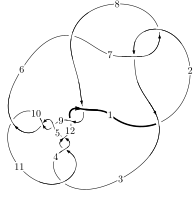
\includegraphics[width=112pt]{../../../GIT/diagram.site/Diagrams/png/1484_12a_0683.png}\\
\ \ \ A knot diagram\footnotemark}&
\allowdisplaybreaks
\textbf{Linearized knot diagam} \\
\cline{2-2}
 &
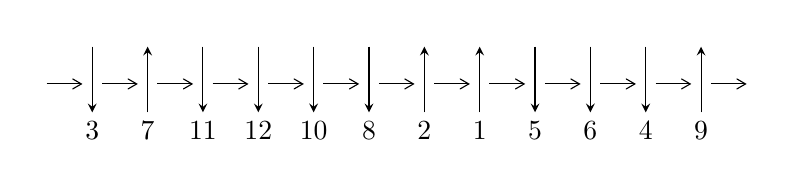
\begin{tikzpicture}[x=20pt, y=17pt]
	% nodes
	\node (C0) at (0, 0) {};
	\node (C1) at (1, 0) {};
	\node (C1U) at (1, +1) {};
	\node (C1D) at (1, -1) {3};

	\node (C2) at (2, 0) {};
	\node (C2U) at (2, +1) {};
	\node (C2D) at (2, -1) {7};

	\node (C3) at (3, 0) {};
	\node (C3U) at (3, +1) {};
	\node (C3D) at (3, -1) {11};

	\node (C4) at (4, 0) {};
	\node (C4U) at (4, +1) {};
	\node (C4D) at (4, -1) {12};

	\node (C5) at (5, 0) {};
	\node (C5U) at (5, +1) {};
	\node (C5D) at (5, -1) {10};

	\node (C6) at (6, 0) {};
	\node (C6U) at (6, +1) {};
	\node (C6D) at (6, -1) {8};

	\node (C7) at (7, 0) {};
	\node (C7U) at (7, +1) {};
	\node (C7D) at (7, -1) {2};

	\node (C8) at (8, 0) {};
	\node (C8U) at (8, +1) {};
	\node (C8D) at (8, -1) {1};

	\node (C9) at (9, 0) {};
	\node (C9U) at (9, +1) {};
	\node (C9D) at (9, -1) {5};

	\node (C10) at (10, 0) {};
	\node (C10U) at (10, +1) {};
	\node (C10D) at (10, -1) {6};

	\node (C11) at (11, 0) {};
	\node (C11U) at (11, +1) {};
	\node (C11D) at (11, -1) {4};

	\node (C12) at (12, 0) {};
	\node (C12U) at (12, +1) {};
	\node (C12D) at (12, -1) {9};
	\node (C13) at (13, 0) {};

	% arrows
	\draw[->,>={angle 60}]
	(C0) edge (C1) (C1) edge (C2) (C2) edge (C3) (C3) edge (C4) (C4) edge (C5) (C5) edge (C6) (C6) edge (C7) (C7) edge (C8) (C8) edge (C9) (C9) edge (C10) (C10) edge (C11) (C11) edge (C12) (C12) edge (C13) ;	\draw[->,>=stealth]
	(C1U) edge (C1D) (C2D) edge (C2U) (C3U) edge (C3D) (C4U) edge (C4D) (C5U) edge (C5D) (C6U) edge (C6D) (C7D) edge (C7U) (C8D) edge (C8U) (C9U) edge (C9D) (C10U) edge (C10D) (C11U) edge (C11D) (C12D) edge (C12U) ;
	\end{tikzpicture} \\
\hhline{~~} \\& 
\textbf{Solving Sequence} \\ \cline{2-2} 
 &
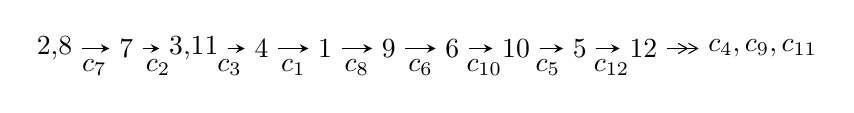
\begin{tikzpicture}[x=23pt, y=7pt]
	% node
	\node (A0) at (-1/8, 0) {2,8};
	\node (A1) at (1, 0) {7};
	\node (A2) at (33/16, 0) {3,11};
	\node (A3) at (25/8, 0) {4};
	\node (A4) at (33/8, 0) {1};
	\node (A5) at (41/8, 0) {9};
	\node (A6) at (49/8, 0) {6};
	\node (A7) at (57/8, 0) {10};
	\node (A8) at (65/8, 0) {5};
	\node (A9) at (73/8, 0) {12};
	\node (C1) at (1/2, -1) {$c_{7}$};
	\node (C2) at (3/2, -1) {$c_{2}$};
	\node (C3) at (21/8, -1) {$c_{3}$};
	\node (C4) at (29/8, -1) {$c_{1}$};
	\node (C5) at (37/8, -1) {$c_{8}$};
	\node (C6) at (45/8, -1) {$c_{6}$};
	\node (C7) at (53/8, -1) {$c_{10}$};
	\node (C8) at (61/8, -1) {$c_{5}$};
	\node (C9) at (69/8, -1) {$c_{12}$};
	\node (A10) at (11, 0) {$c_{4},c_{9},c_{11}$};

	% edge
	\draw[->,>=stealth]	
	(A0) edge (A1) (A1) edge (A2) (A2) edge (A3) (A3) edge (A4) (A4) edge (A5) (A5) edge (A6) (A6) edge (A7) (A7) edge (A8) (A8) edge (A9) ;
	\draw[->>,>={angle 60}]	
	(A9) edge (A10);
\end{tikzpicture} \\ 

\end{tabular} \\

\footnotetext{
The image of knot diagram is generated by the software ``\textbf{Draw programme}" developed by Andrew Bartholomew(\url{http://www.layer8.co.uk/maths/draw/index.htm\#Running-draw}), where we modified some parts for our purpose(\url{https://github.com/CATsTAILs/LinksPainter}).
}\phantom \\ \newline 
\centering \textbf{Ideals for irreducible components\footnotemark of $X_{\text{par}}$} 
 
\begin{align*}
I^u_{1}&=\langle 
4 u^{29}-7 u^{28}+\cdots+b+7,\;-7 u^{30}+21 u^{29}+\cdots+2 a+16,\;u^{31}-3 u^{30}+\cdots+2 u+2\rangle \\
I^u_{2}&=\langle 
- u^{18}- u^{17}+\cdots+b-1,\;- u^{18} a- u^{18}+\cdots- a-1,\;u^{19}+u^{18}+\cdots+2 u-1\rangle \\
I^u_{3}&=\langle 
- u^2+b- u-1,\;u^3+2 a- u-2,\;u^4+u^2+2\rangle \\
I^u_{4}&=\langle 
b+u,\;a+1,\;u^2+1\rangle \\
I^u_{5}&=\langle 
u^3+u^2+b-1,\;u^3+u^2+a+u,\;u^4+1\rangle \\
\\
I^v_{1}&=\langle 
a,\;b-1,\;v+1\rangle \\
\end{align*}
\raggedright * 6 irreducible components of $\dim_{\mathbb{C}}=0$, with total 80 representations.\\
\footnotetext{All coefficients of polynomials are rational numbers. But the coefficients are sometimes approximated in decimal forms when there is not enough margin.}
\newpage
\renewcommand{\arraystretch}{1}
\centering \section*{I. $I^u_{1}= \langle 4 u^{29}-7 u^{28}+\cdots+b+7,\;-7 u^{30}+21 u^{29}+\cdots+2 a+16,\;u^{31}-3 u^{30}+\cdots+2 u+2 \rangle$}
\flushleft \textbf{(i) Arc colorings}\\
\begin{tabular}{m{7pt} m{180pt} m{7pt} m{180pt} }
\flushright $a_{2}=$&$\begin{pmatrix}0\\u\end{pmatrix}$ \\
\flushright $a_{8}=$&$\begin{pmatrix}1\\0\end{pmatrix}$ \\
\flushright $a_{7}=$&$\begin{pmatrix}1\\u^2\end{pmatrix}$ \\
\flushright $a_{3}=$&$\begin{pmatrix}u\\u^3+u\end{pmatrix}$ \\
\flushright $a_{11}=$&$\begin{pmatrix}\frac{7}{2} u^{30}-\frac{21}{2} u^{29}+\cdots-13 u-8\\-4 u^{29}+7 u^{28}+\cdots-15 u-7\end{pmatrix}$ \\
\flushright $a_{4}=$&$\begin{pmatrix}-\frac{1}{2} u^{30}+\frac{1}{2} u^{29}+\cdots+u^2+u\\- u^{30}+2 u^{29}+\cdots+2 u+1\end{pmatrix}$ \\
\flushright $a_{1}=$&$\begin{pmatrix}u^3\\u^5+u^3+u\end{pmatrix}$ \\
\flushright $a_{9}=$&$\begin{pmatrix}- u^8- u^6- u^4+1\\- u^{10}-2 u^8-3 u^6-2 u^4- u^2\end{pmatrix}$ \\
\flushright $a_{6}=$&$\begin{pmatrix}u^2+1\\u^2\end{pmatrix}$ \\
\flushright $a_{10}=$&$\begin{pmatrix}\frac{5}{2} u^{30}-\frac{15}{2} u^{29}+\cdots-9 u-5\\-3 u^{29}+5 u^{28}+\cdots-11 u-5\end{pmatrix}$ \\
\flushright $a_{5}=$&$\begin{pmatrix}\frac{3}{2} u^{30}-\frac{5}{2} u^{29}+\cdots+\frac{15}{2} u^3+u^2\\u^{30}-2 u^{29}+\cdots- u-1\end{pmatrix}$ \\
\flushright $a_{12}=$&$\begin{pmatrix}u^{13}+2 u^{11}+3 u^9+2 u^7- u\\u^{15}+3 u^{13}+6 u^{11}+7 u^9+6 u^7+4 u^5+2 u^3+u\end{pmatrix}$\\&\end{tabular}
\flushleft \textbf{(ii) Obstruction class $= -1$}\\~\\
\flushleft \textbf{(iii) Cusp Shapes $= -2 u^{30}+8 u^{29}-18 u^{28}+42 u^{27}-66 u^{26}+130 u^{25}-152 u^{24}+264 u^{23}-238 u^{22}+400 u^{21}-254 u^{20}+478 u^{19}-184 u^{18}+486 u^{17}-50 u^{16}+466 u^{15}+62 u^{14}+410 u^{13}+144 u^{12}+350 u^{11}+186 u^{10}+252 u^9+162 u^8+174 u^7+138 u^6+104 u^5+80 u^4+36 u^3+40 u^2+34 u+8$}\\~\\
\newpage\renewcommand{\arraystretch}{1}
\flushleft \textbf{(iv) u-Polynomials at the component}\newline \\
\begin{tabular}{m{50pt}|m{274pt}}
Crossings & \hspace{64pt}u-Polynomials at each crossing \\
\hline $$\begin{aligned}c_{1},c_{6}\end{aligned}$$&$\begin{aligned}
&u^{31}+11 u^{30}+\cdots-28 u-4
\end{aligned}$\\
\hline $$\begin{aligned}c_{2},c_{7}\end{aligned}$$&$\begin{aligned}
&u^{31}+3 u^{30}+\cdots+2 u-2
\end{aligned}$\\
\hline $$\begin{aligned}c_{3},c_{4},c_{5}\\c_{9},c_{10},c_{11}\end{aligned}$$&$\begin{aligned}
&u^{31}+u^{30}+\cdots+2 u+1
\end{aligned}$\\
\hline $$\begin{aligned}c_{8},c_{12}\end{aligned}$$&$\begin{aligned}
&u^{31}-15 u^{30}+\cdots+3142 u-314
\end{aligned}$\\
\hline
\end{tabular}\\~\\
\newpage\renewcommand{\arraystretch}{1}
\flushleft \textbf{(v) Riley Polynomials at the component}\newline \\
\begin{tabular}{m{50pt}|m{274pt}}
Crossings & \hspace{64pt}Riley Polynomials at each crossing \\
\hline $$\begin{aligned}c_{1},c_{6}\end{aligned}$$&$\begin{aligned}
&y^{31}+19 y^{30}+\cdots-336 y-16
\end{aligned}$\\
\hline $$\begin{aligned}c_{2},c_{7}\end{aligned}$$&$\begin{aligned}
&y^{31}+11 y^{30}+\cdots-28 y-4
\end{aligned}$\\
\hline $$\begin{aligned}c_{3},c_{4},c_{5}\\c_{9},c_{10},c_{11}\end{aligned}$$&$\begin{aligned}
&y^{31}-41 y^{30}+\cdots+6 y-1
\end{aligned}$\\
\hline $$\begin{aligned}c_{8},c_{12}\end{aligned}$$&$\begin{aligned}
&y^{31}+23 y^{30}+\cdots-1185660 y-98596
\end{aligned}$\\
\hline
\end{tabular}\\~\\
\newpage\flushleft \textbf{(vi) Complex Volumes and Cusp Shapes}
$$\begin{array}{c|c|c}  
\text{Solutions to }I^u_{1}& \I (\text{vol} + \sqrt{-1}CS) & \text{Cusp shape}\\
 \hline 
\begin{aligned}
u &= \phantom{-}0.834590 + 0.582027 I \\
a &= -1.21990 + 2.11129 I \\
b &= -2.24694 + 1.05205 I\end{aligned}
 & -12.7225 - 9.0086 I & -8.83881 + 3.40935 I \\ \hline\begin{aligned}
u &= \phantom{-}0.834590 - 0.582027 I \\
a &= -1.21990 - 2.11129 I \\
b &= -2.24694 - 1.05205 I\end{aligned}
 & -12.7225 + 9.0086 I & -8.83881 - 3.40935 I \\ \hline\begin{aligned}
u &= \phantom{-}0.722502 + 0.621547 I \\
a &= \phantom{-}1.250200 - 0.565257 I \\
b &= \phantom{-}1.254610 + 0.368661 I\end{aligned}
 & \phantom{-}0.64783 - 2.08671 I & -2.33564 + 4.90914 I \\ \hline\begin{aligned}
u &= \phantom{-}0.722502 - 0.621547 I \\
a &= \phantom{-}1.250200 + 0.565257 I \\
b &= \phantom{-}1.254610 - 0.368661 I\end{aligned}
 & \phantom{-}0.64783 + 2.08671 I & -2.33564 - 4.90914 I \\ \hline\begin{aligned}
u &= -0.011192 + 1.055950 I \\
a &= -0.403491 - 0.377694 I \\
b &= \phantom{-}0.403341 - 0.421839 I\end{aligned}
 & -4.70000 - 1.40560 I & -10.10684 + 4.97569 I \\ \hline\begin{aligned}
u &= -0.011192 - 1.055950 I \\
a &= -0.403491 + 0.377694 I \\
b &= \phantom{-}0.403341 + 0.421839 I\end{aligned}
 & -4.70000 + 1.40560 I & -10.10684 - 4.97569 I \\ \hline\begin{aligned}
u &= -0.660425 + 0.655957 I \\
a &= \phantom{-}0.095218 - 0.222295 I \\
b &= \phantom{-}0.082932 + 0.209267 I\end{aligned}
 & \phantom{-}0.242168 - 0.690936 I & -4.10470 + 4.18335 I \\ \hline\begin{aligned}
u &= -0.660425 - 0.655957 I \\
a &= \phantom{-}0.095218 + 0.222295 I \\
b &= \phantom{-}0.082932 - 0.209267 I\end{aligned}
 & \phantom{-}0.242168 + 0.690936 I & -4.10470 - 4.18335 I \\ \hline\begin{aligned}
u &= -0.317662 + 1.028560 I \\
a &= -0.763693 + 0.390412 I \\
b &= -0.158967 - 0.909525 I\end{aligned}
 & -12.44600 - 3.27738 I & -13.9945 + 3.6592 I \\ \hline\begin{aligned}
u &= -0.317662 - 1.028560 I \\
a &= -0.763693 - 0.390412 I \\
b &= -0.158967 + 0.909525 I\end{aligned}
 & -12.44600 + 3.27738 I & -13.9945 - 3.6592 I\\
 \hline 
 \end{array}$$\newpage$$\begin{array}{c|c|c}  
\text{Solutions to }I^u_{1}& \I (\text{vol} + \sqrt{-1}CS) & \text{Cusp shape}\\
 \hline 
\begin{aligned}
u &= \phantom{-}0.688487 + 0.854024 I \\
a &= -1.32554 + 1.02312 I \\
b &= -1.78639 - 0.42763 I\end{aligned}
 & \phantom{-}3.47574 + 2.64776 I & \phantom{-}2.40040 - 3.76300 I \\ \hline\begin{aligned}
u &= \phantom{-}0.688487 - 0.854024 I \\
a &= -1.32554 - 1.02312 I \\
b &= -1.78639 + 0.42763 I\end{aligned}
 & \phantom{-}3.47574 - 2.64776 I & \phantom{-}2.40040 + 3.76300 I \\ \hline\begin{aligned}
u &= \phantom{-}0.806865 + 0.777962 I \\
a &= -0.57745 - 2.39117 I \\
b &= \phantom{-}1.39431 - 2.37858 I\end{aligned}
 & -5.26559 - 1.70254 I & -7.93225 + 0.49720 I \\ \hline\begin{aligned}
u &= \phantom{-}0.806865 - 0.777962 I \\
a &= -0.57745 + 2.39117 I \\
b &= \phantom{-}1.39431 + 2.37858 I\end{aligned}
 & -5.26559 + 1.70254 I & -7.93225 - 0.49720 I \\ \hline\begin{aligned}
u &= -0.772524 + 0.407584 I \\
a &= \phantom{-}0.357260 + 0.680444 I \\
b &= -0.553330 - 0.380046 I\end{aligned}
 & -13.7371 - 5.6675 I & -9.37862 + 3.30798 I \\ \hline\begin{aligned}
u &= -0.772524 - 0.407584 I \\
a &= \phantom{-}0.357260 - 0.680444 I \\
b &= -0.553330 + 0.380046 I\end{aligned}
 & -13.7371 + 5.6675 I & -9.37862 - 3.30798 I \\ \hline\begin{aligned}
u &= -0.062033 + 1.149980 I \\
a &= \phantom{-}1.032410 + 0.353539 I \\
b &= -0.470604 + 1.165310 I\end{aligned}
 & -19.0694 - 7.7866 I & -15.0141 + 3.7811 I \\ \hline\begin{aligned}
u &= -0.062033 - 1.149980 I \\
a &= \phantom{-}1.032410 - 0.353539 I \\
b &= -0.470604 - 1.165310 I\end{aligned}
 & -19.0694 + 7.7866 I & -15.0141 - 3.7811 I \\ \hline\begin{aligned}
u &= -0.655738 + 0.995207 I \\
a &= -0.016249 + 0.192084 I \\
b &= -0.180508 - 0.142129 I\end{aligned}
 & -0.76854 - 4.47807 I & -5.49078 + 0.99191 I \\ \hline\begin{aligned}
u &= -0.655738 - 0.995207 I \\
a &= -0.016249 - 0.192084 I \\
b &= -0.180508 + 0.142129 I\end{aligned}
 & -0.76854 + 4.47807 I & -5.49078 - 0.99191 I\\
 \hline 
 \end{array}$$\newpage$$\begin{array}{c|c|c}  
\text{Solutions to }I^u_{1}& \I (\text{vol} + \sqrt{-1}CS) & \text{Cusp shape}\\
 \hline 
\begin{aligned}
u &= \phantom{-}0.663735 + 1.013080 I \\
a &= \phantom{-}0.869119 - 1.080960 I \\
b &= \phantom{-}1.67196 + 0.16301 I\end{aligned}
 & -0.50643 + 7.41412 I & -4.69631 - 9.68387 I \\ \hline\begin{aligned}
u &= \phantom{-}0.663735 - 1.013080 I \\
a &= \phantom{-}0.869119 + 1.080960 I \\
b &= \phantom{-}1.67196 - 0.16301 I\end{aligned}
 & -0.50643 - 7.41412 I & -4.69631 + 9.68387 I \\ \hline\begin{aligned}
u &= \phantom{-}0.755579 + 0.953754 I \\
a &= \phantom{-}2.25812 + 0.93449 I \\
b &= \phantom{-}0.81492 + 2.85977 I\end{aligned}
 & -5.80221 + 7.55915 I & -8.80311 - 5.88769 I \\ \hline\begin{aligned}
u &= \phantom{-}0.755579 - 0.953754 I \\
a &= \phantom{-}2.25812 - 0.93449 I \\
b &= \phantom{-}0.81492 - 2.85977 I\end{aligned}
 & -5.80221 - 7.55915 I & -8.80311 + 5.88769 I \\ \hline\begin{aligned}
u &= -0.598928 + 1.072520 I \\
a &= \phantom{-}0.297943 - 0.455847 I \\
b &= \phantom{-}0.310457 + 0.592568 I\end{aligned}
 & -15.6742 + 0.5629 I & -12.28287 + 1.51453 I \\ \hline\begin{aligned}
u &= -0.598928 - 1.072520 I \\
a &= \phantom{-}0.297943 + 0.455847 I \\
b &= \phantom{-}0.310457 - 0.592568 I\end{aligned}
 & -15.6742 - 0.5629 I & -12.28287 - 1.51453 I \\ \hline\begin{aligned}
u &= \phantom{-}0.689812 + 1.062820 I \\
a &= -2.28466 + 0.81265 I \\
b &= -2.43969 - 1.86761 I\end{aligned}
 & -14.1718 + 14.7070 I & -10.75887 - 7.88304 I \\ \hline\begin{aligned}
u &= \phantom{-}0.689812 - 1.062820 I \\
a &= -2.28466 - 0.81265 I \\
b &= -2.43969 + 1.86761 I\end{aligned}
 & -14.1718 - 14.7070 I & -10.75887 + 7.88304 I \\ \hline\begin{aligned}
u &= -0.671467\phantom{ +0.000000I} \\
a &= -1.07798\phantom{ +0.000000I} \\
b &= \phantom{-}0.723830\phantom{ +0.000000I}\end{aligned}
 & -9.27702\phantom{ +0.000000I} & -8.24970\phantom{ +0.000000I} \\ \hline\begin{aligned}
u &= -0.247335 + 0.431598 I \\
a &= \phantom{-}0.469701 - 0.366440 I \\
b &= \phantom{-}0.041981 + 0.293355 I\end{aligned}
 & -0.139351 - 0.826891 I & -3.53813 + 8.27499 I\\
 \hline 
 \end{array}$$\newpage$$\begin{array}{c|c|c}  
\text{Solutions to }I^u_{1}& \I (\text{vol} + \sqrt{-1}CS) & \text{Cusp shape}\\
 \hline 
\begin{aligned}
u &= -0.247335 - 0.431598 I \\
a &= \phantom{-}0.469701 + 0.366440 I \\
b &= \phantom{-}0.041981 - 0.293355 I\end{aligned}
 & -0.139351 + 0.826891 I & -3.53813 - 8.27499 I\\
 \hline 
 \end{array}$$\newpage\newpage\renewcommand{\arraystretch}{1}
\centering \section*{II. $I^u_{2}= \langle - u^{18}- u^{17}+\cdots+b-1,\;- u^{18} a- u^{18}+\cdots- a-1,\;u^{19}+u^{18}+\cdots+2 u-1 \rangle$}
\flushleft \textbf{(i) Arc colorings}\\
\begin{tabular}{m{7pt} m{180pt} m{7pt} m{180pt} }
\flushright $a_{2}=$&$\begin{pmatrix}0\\u\end{pmatrix}$ \\
\flushright $a_{8}=$&$\begin{pmatrix}1\\0\end{pmatrix}$ \\
\flushright $a_{7}=$&$\begin{pmatrix}1\\u^2\end{pmatrix}$ \\
\flushright $a_{3}=$&$\begin{pmatrix}u\\u^3+u\end{pmatrix}$ \\
\flushright $a_{11}=$&$\begin{pmatrix}a\\u^{18}+u^{17}+\cdots- u+1\end{pmatrix}$ \\
\flushright $a_{4}=$&$\begin{pmatrix}u^{18}+u^{17}+\cdots- a+2 u\\u^{18} a+u^{17} a+\cdots+u+1\end{pmatrix}$ \\
\flushright $a_{1}=$&$\begin{pmatrix}u^3\\u^5+u^3+u\end{pmatrix}$ \\
\flushright $a_{9}=$&$\begin{pmatrix}- u^8- u^6- u^4+1\\- u^{10}-2 u^8-3 u^6-2 u^4- u^2\end{pmatrix}$ \\
\flushright $a_{6}=$&$\begin{pmatrix}u^2+1\\u^2\end{pmatrix}$ \\
\flushright $a_{10}=$&$\begin{pmatrix}- u^{18}- u^{17}+\cdots+a+1\\u^{14}+u^{13}+\cdots- u+1\end{pmatrix}$ \\
\flushright $a_{5}=$&$\begin{pmatrix}- u^{18}- u^{17}+\cdots+a- u\\2 u^{16}+2 u^{15}+\cdots- u-1\end{pmatrix}$ \\
\flushright $a_{12}=$&$\begin{pmatrix}u^{13}+2 u^{11}+3 u^9+2 u^7- u\\u^{15}+3 u^{13}+6 u^{11}+7 u^9+6 u^7+4 u^5+2 u^3+u\end{pmatrix}$\\&\end{tabular}
\flushleft \textbf{(ii) Obstruction class $= -1$}\\~\\
\flushleft \textbf{(iii) Cusp Shapes $= 4 u^{17}+4 u^{16}+12 u^{15}+12 u^{14}+28 u^{13}+24 u^{12}+36 u^{11}+32 u^{10}+36 u^9+28 u^8+28 u^7+28 u^6+12 u^5+16 u^4+12 u^3+12 u^2-4 u-2$}\\~\\
\newpage\renewcommand{\arraystretch}{1}
\flushleft \textbf{(iv) u-Polynomials at the component}\newline \\
\begin{tabular}{m{50pt}|m{274pt}}
Crossings & \hspace{64pt}u-Polynomials at each crossing \\
\hline $$\begin{aligned}c_{1},c_{6}\end{aligned}$$&$\begin{aligned}
&(u^{19}+7 u^{18}+\cdots+2 u-1)^{2}
\end{aligned}$\\
\hline $$\begin{aligned}c_{2},c_{7}\end{aligned}$$&$\begin{aligned}
&(u^{19}- u^{18}+\cdots+2 u+1)^{2}
\end{aligned}$\\
\hline $$\begin{aligned}c_{3},c_{4},c_{5}\\c_{9},c_{10},c_{11}\end{aligned}$$&$\begin{aligned}
&u^{38}+u^{37}+\cdots+11 u-16
\end{aligned}$\\
\hline $$\begin{aligned}c_{8},c_{12}\end{aligned}$$&$\begin{aligned}
&(u^{19}+5 u^{18}+\cdots+2 u+1)^{2}
\end{aligned}$\\
\hline
\end{tabular}\\~\\
\newpage\renewcommand{\arraystretch}{1}
\flushleft \textbf{(v) Riley Polynomials at the component}\newline \\
\begin{tabular}{m{50pt}|m{274pt}}
Crossings & \hspace{64pt}Riley Polynomials at each crossing \\
\hline $$\begin{aligned}c_{1},c_{6}\end{aligned}$$&$\begin{aligned}
&(y^{19}+11 y^{18}+\cdots+42 y-1)^{2}
\end{aligned}$\\
\hline $$\begin{aligned}c_{2},c_{7}\end{aligned}$$&$\begin{aligned}
&(y^{19}+7 y^{18}+\cdots+2 y-1)^{2}
\end{aligned}$\\
\hline $$\begin{aligned}c_{3},c_{4},c_{5}\\c_{9},c_{10},c_{11}\end{aligned}$$&$\begin{aligned}
&y^{38}-33 y^{37}+\cdots-153 y+256
\end{aligned}$\\
\hline $$\begin{aligned}c_{8},c_{12}\end{aligned}$$&$\begin{aligned}
&(y^{19}+19 y^{18}+\cdots+10 y-1)^{2}
\end{aligned}$\\
\hline
\end{tabular}\\~\\
\newpage\flushleft \textbf{(vi) Complex Volumes and Cusp Shapes}
$$\begin{array}{c|c|c}  
\text{Solutions to }I^u_{2}& \I (\text{vol} + \sqrt{-1}CS) & \text{Cusp shape}\\
 \hline 
\begin{aligned}
u &= -0.787239 + 0.559366 I \\
a &= -1.59518 - 1.01906 I \\
b &= -1.96110 - 0.37239 I\end{aligned}
 & -5.72757 + 4.39903 I & -7.06652 - 2.80289 I \\ \hline\begin{aligned}
u &= -0.787239 + 0.559366 I \\
a &= \phantom{-}1.43202 + 1.49055 I \\
b &= \phantom{-}1.82582 - 0.09005 I\end{aligned}
 & -5.72757 + 4.39903 I & -7.06652 - 2.80289 I \\ \hline\begin{aligned}
u &= -0.787239 - 0.559366 I \\
a &= -1.59518 + 1.01906 I \\
b &= -1.96110 + 0.37239 I\end{aligned}
 & -5.72757 - 4.39903 I & -7.06652 + 2.80289 I \\ \hline\begin{aligned}
u &= -0.787239 - 0.559366 I \\
a &= \phantom{-}1.43202 - 1.49055 I \\
b &= \phantom{-}1.82582 + 0.09005 I\end{aligned}
 & -5.72757 - 4.39903 I & -7.06652 + 2.80289 I \\ \hline\begin{aligned}
u &= -0.709462 + 0.766103 I \\
a &= \phantom{-}0.29719 + 1.53619 I \\
b &= \phantom{-}1.57544 + 1.21787 I\end{aligned}
 & \phantom{-}0.332249 + 0.168160 I & -1.83171 - 0.91431 I \\ \hline\begin{aligned}
u &= -0.709462 + 0.766103 I \\
a &= -0.16941 - 1.89955 I \\
b &= -1.38773 - 0.86219 I\end{aligned}
 & \phantom{-}0.332249 + 0.168160 I & -1.83171 - 0.91431 I \\ \hline\begin{aligned}
u &= -0.709462 - 0.766103 I \\
a &= \phantom{-}0.29719 - 1.53619 I \\
b &= \phantom{-}1.57544 - 1.21787 I\end{aligned}
 & \phantom{-}0.332249 - 0.168160 I & -1.83171 + 0.91431 I \\ \hline\begin{aligned}
u &= -0.709462 - 0.766103 I \\
a &= -0.16941 + 1.89955 I \\
b &= -1.38773 + 0.86219 I\end{aligned}
 & \phantom{-}0.332249 - 0.168160 I & -1.83171 + 0.91431 I \\ \hline\begin{aligned}
u &= \phantom{-}0.588600 + 0.865037 I \\
a &= \phantom{-}1.55445 - 0.80251 I \\
b &= \phantom{-}2.17659 + 0.04078 I\end{aligned}
 & -2.82151 + 2.32534 I & -9.72826 - 3.09456 I \\ \hline\begin{aligned}
u &= \phantom{-}0.588600 + 0.865037 I \\
a &= \phantom{-}1.20249 - 1.69796 I \\
b &= \phantom{-}1.60915 + 0.87230 I\end{aligned}
 & -2.82151 + 2.32534 I & -9.72826 - 3.09456 I\\
 \hline 
 \end{array}$$\newpage$$\begin{array}{c|c|c}  
\text{Solutions to }I^u_{2}& \I (\text{vol} + \sqrt{-1}CS) & \text{Cusp shape}\\
 \hline 
\begin{aligned}
u &= \phantom{-}0.588600 - 0.865037 I \\
a &= \phantom{-}1.55445 + 0.80251 I \\
b &= \phantom{-}2.17659 - 0.04078 I\end{aligned}
 & -2.82151 - 2.32534 I & -9.72826 + 3.09456 I \\ \hline\begin{aligned}
u &= \phantom{-}0.588600 - 0.865037 I \\
a &= \phantom{-}1.20249 + 1.69796 I \\
b &= \phantom{-}1.60915 - 0.87230 I\end{aligned}
 & -2.82151 - 2.32534 I & -9.72826 + 3.09456 I \\ \hline\begin{aligned}
u &= \phantom{-}0.745489 + 0.500016 I \\
a &= -0.996497 - 0.309724 I \\
b &= -1.167150 + 0.064986 I\end{aligned}
 & -6.12368 + 1.53005 I & -7.79395 - 2.54963 I \\ \hline\begin{aligned}
u &= \phantom{-}0.745489 + 0.500016 I \\
a &= -1.039500 + 0.784391 I \\
b &= -0.588010 - 0.729160 I\end{aligned}
 & -6.12368 + 1.53005 I & -7.79395 - 2.54963 I \\ \hline\begin{aligned}
u &= \phantom{-}0.745489 - 0.500016 I \\
a &= -0.996497 + 0.309724 I \\
b &= -1.167150 - 0.064986 I\end{aligned}
 & -6.12368 - 1.53005 I & -7.79395 + 2.54963 I \\ \hline\begin{aligned}
u &= \phantom{-}0.745489 - 0.500016 I \\
a &= -1.039500 - 0.784391 I \\
b &= -0.588010 + 0.729160 I\end{aligned}
 & -6.12368 - 1.53005 I & -7.79395 + 2.54963 I \\ \hline\begin{aligned}
u &= \phantom{-}0.021471 + 1.128170 I \\
a &= \phantom{-}0.965139 - 0.110361 I \\
b &= -1.080140 - 0.504142 I\end{aligned}
 & -11.59750 + 3.11880 I & -13.58624 - 2.69239 I \\ \hline\begin{aligned}
u &= \phantom{-}0.021471 + 1.128170 I \\
a &= -0.464921 + 0.948575 I \\
b &= \phantom{-}0.145228 + 1.086470 I\end{aligned}
 & -11.59750 + 3.11880 I & -13.58624 - 2.69239 I \\ \hline\begin{aligned}
u &= \phantom{-}0.021471 - 1.128170 I \\
a &= \phantom{-}0.965139 + 0.110361 I \\
b &= -1.080140 + 0.504142 I\end{aligned}
 & -11.59750 - 3.11880 I & -13.58624 + 2.69239 I \\ \hline\begin{aligned}
u &= \phantom{-}0.021471 - 1.128170 I \\
a &= -0.464921 - 0.948575 I \\
b &= \phantom{-}0.145228 - 1.086470 I\end{aligned}
 & -11.59750 - 3.11880 I & -13.58624 + 2.69239 I\\
 \hline 
 \end{array}$$\newpage$$\begin{array}{c|c|c}  
\text{Solutions to }I^u_{2}& \I (\text{vol} + \sqrt{-1}CS) & \text{Cusp shape}\\
 \hline 
\begin{aligned}
u &= \phantom{-}0.167515 + 0.839557 I \\
a &= -1.53925 - 0.74620 I \\
b &= \phantom{-}0.085530 + 0.151965 I\end{aligned}
 & -4.70093 + 1.72326 I & -11.81965 - 5.18112 I \\ \hline\begin{aligned}
u &= \phantom{-}0.167515 + 0.839557 I \\
a &= \phantom{-}0.193624 - 0.063242 I \\
b &= \phantom{-}0.36863 - 1.41729 I\end{aligned}
 & -4.70093 + 1.72326 I & -11.81965 - 5.18112 I \\ \hline\begin{aligned}
u &= \phantom{-}0.167515 - 0.839557 I \\
a &= -1.53925 + 0.74620 I \\
b &= \phantom{-}0.085530 - 0.151965 I\end{aligned}
 & -4.70093 - 1.72326 I & -11.81965 + 5.18112 I \\ \hline\begin{aligned}
u &= \phantom{-}0.167515 - 0.839557 I \\
a &= \phantom{-}0.193624 + 0.063242 I \\
b &= \phantom{-}0.36863 + 1.41729 I\end{aligned}
 & -4.70093 - 1.72326 I & -11.81965 + 5.18112 I \\ \hline\begin{aligned}
u &= -0.687512 + 0.928828 I \\
a &= \phantom{-}1.83316 + 0.24348 I \\
b &= \phantom{-}1.18697 - 1.80258 I\end{aligned}
 & -0.16029 - 5.52702 I & -3.57206 + 7.00248 I \\ \hline\begin{aligned}
u &= -0.687512 + 0.928828 I \\
a &= -1.86487 + 0.10244 I \\
b &= -1.48646 + 1.53530 I\end{aligned}
 & -0.16029 - 5.52702 I & -3.57206 + 7.00248 I \\ \hline\begin{aligned}
u &= -0.687512 - 0.928828 I \\
a &= \phantom{-}1.83316 - 0.24348 I \\
b &= \phantom{-}1.18697 + 1.80258 I\end{aligned}
 & -0.16029 + 5.52702 I & -3.57206 - 7.00248 I \\ \hline\begin{aligned}
u &= -0.687512 - 0.928828 I \\
a &= -1.86487 - 0.10244 I \\
b &= -1.48646 - 1.53530 I\end{aligned}
 & -0.16029 + 5.52702 I & -3.57206 - 7.00248 I \\ \hline\begin{aligned}
u &= \phantom{-}0.636878 + 1.050560 I \\
a &= -0.563849 + 0.610645 I \\
b &= -1.65719 + 0.48350 I\end{aligned}
 & -7.70394 + 3.71612 I & -10.19900 - 2.45937 I \\ \hline\begin{aligned}
u &= \phantom{-}0.636878 + 1.050560 I \\
a &= -0.362743 + 1.357530 I \\
b &= -1.000620 - 0.203449 I\end{aligned}
 & -7.70394 + 3.71612 I & -10.19900 - 2.45937 I\\
 \hline 
 \end{array}$$\newpage$$\begin{array}{c|c|c}  
\text{Solutions to }I^u_{2}& \I (\text{vol} + \sqrt{-1}CS) & \text{Cusp shape}\\
 \hline 
\begin{aligned}
u &= \phantom{-}0.636878 - 1.050560 I \\
a &= -0.563849 - 0.610645 I \\
b &= -1.65719 - 0.48350 I\end{aligned}
 & -7.70394 - 3.71612 I & -10.19900 + 2.45937 I \\ \hline\begin{aligned}
u &= \phantom{-}0.636878 - 1.050560 I \\
a &= -0.362743 - 1.357530 I \\
b &= -1.000620 + 0.203449 I\end{aligned}
 & -7.70394 - 3.71612 I & -10.19900 + 2.45937 I \\ \hline\begin{aligned}
u &= -0.666721 + 1.052350 I \\
a &= \phantom{-}1.51291 + 1.05726 I \\
b &= \phantom{-}2.53933 - 0.66065 I\end{aligned}
 & -7.18622 - 9.88550 I & -9.13872 + 7.31129 I \\ \hline\begin{aligned}
u &= -0.666721 + 1.052350 I \\
a &= -1.53887 - 1.43806 I \\
b &= -2.12129 + 0.88721 I\end{aligned}
 & -7.18622 - 9.88550 I & -9.13872 + 7.31129 I \\ \hline\begin{aligned}
u &= -0.666721 - 1.052350 I \\
a &= \phantom{-}1.51291 - 1.05726 I \\
b &= \phantom{-}2.53933 + 0.66065 I\end{aligned}
 & -7.18622 + 9.88550 I & -9.13872 - 7.31129 I \\ \hline\begin{aligned}
u &= -0.666721 - 1.052350 I \\
a &= -1.53887 + 1.43806 I \\
b &= -2.12129 - 0.88721 I\end{aligned}
 & -7.18622 + 9.88550 I & -9.13872 - 7.31129 I \\ \hline\begin{aligned}
u &= \phantom{-}0.381963\phantom{ +0.000000I} \\
a &= -0.253895\phantom{ +0.000000I} \\
b &= \phantom{-}0.971005\phantom{ +0.000000I}\end{aligned}
 & -2.38250\phantom{ +0.000000I} & -0.527780\phantom{ +0.000000I} \\ \hline\begin{aligned}
u &= \phantom{-}0.381963\phantom{ +0.000000I} \\
a &= \phantom{-}2.54214\phantom{ +0.000000I} \\
b &= -0.0969785\phantom{ +0.000000I}\end{aligned}
 & -2.38250\phantom{ +0.000000I} & -0.527780\phantom{ +0.000000I}\\
 \hline 
 \end{array}$$\newpage\newpage\renewcommand{\arraystretch}{1}
\centering \section*{III. $I^u_{3}= \langle - u^2+b- u-1,\;u^3+2 a- u-2,\;u^4+u^2+2 \rangle$}
\flushleft \textbf{(i) Arc colorings}\\
\begin{tabular}{m{7pt} m{180pt} m{7pt} m{180pt} }
\flushright $a_{2}=$&$\begin{pmatrix}0\\u\end{pmatrix}$ \\
\flushright $a_{8}=$&$\begin{pmatrix}1\\0\end{pmatrix}$ \\
\flushright $a_{7}=$&$\begin{pmatrix}1\\u^2\end{pmatrix}$ \\
\flushright $a_{3}=$&$\begin{pmatrix}u\\u^3+u\end{pmatrix}$ \\
\flushright $a_{11}=$&$\begin{pmatrix}-\frac{1}{2} u^3+\frac{1}{2} u+1\\u^2+u+1\end{pmatrix}$ \\
\flushright $a_{4}=$&$\begin{pmatrix}-\frac{1}{2} u^3+\frac{3}{2} u+1\\u^3+u^2+2 u+1\end{pmatrix}$ \\
\flushright $a_{1}=$&$\begin{pmatrix}u^3\\- u\end{pmatrix}$ \\
\flushright $a_{9}=$&$\begin{pmatrix}- u^2-1\\- u^2\end{pmatrix}$ \\
\flushright $a_{6}=$&$\begin{pmatrix}u^2+1\\u^2\end{pmatrix}$ \\
\flushright $a_{10}=$&$\begin{pmatrix}-\frac{1}{2} u^3- u^2+\frac{1}{2} u\\u+1\end{pmatrix}$ \\
\flushright $a_{5}=$&$\begin{pmatrix}-\frac{1}{2} u^3+\frac{1}{2} u+1\\u^2+u+1\end{pmatrix}$ \\
\flushright $a_{12}=$&$\begin{pmatrix}- u\\- u^3- u\end{pmatrix}$\\&\end{tabular}
\flushleft \textbf{(ii) Obstruction class $= 1$}\\~\\
\flushleft \textbf{(iii) Cusp Shapes $= -4 u^2-12$}\\~\\
\newpage\renewcommand{\arraystretch}{1}
\flushleft \textbf{(iv) u-Polynomials at the component}\newline \\
\begin{tabular}{m{50pt}|m{274pt}}
Crossings & \hspace{64pt}u-Polynomials at each crossing \\
\hline $$\begin{aligned}c_{1},c_{6}\end{aligned}$$&$\begin{aligned}
&(u^2- u+2)^2
\end{aligned}$\\
\hline $$\begin{aligned}c_{2},c_{7},c_{8}\\c_{12}\end{aligned}$$&$\begin{aligned}
&u^4+u^2+2
\end{aligned}$\\
\hline $$\begin{aligned}c_{3},c_{4},c_{9}\\c_{10}\end{aligned}$$&$\begin{aligned}
&(u-1)^4
\end{aligned}$\\
\hline $$\begin{aligned}c_{5},c_{11}\end{aligned}$$&$\begin{aligned}
&(u+1)^4
\end{aligned}$\\
\hline
\end{tabular}\\~\\
\newpage\renewcommand{\arraystretch}{1}
\flushleft \textbf{(v) Riley Polynomials at the component}\newline \\
\begin{tabular}{m{50pt}|m{274pt}}
Crossings & \hspace{64pt}Riley Polynomials at each crossing \\
\hline $$\begin{aligned}c_{1},c_{6}\end{aligned}$$&$\begin{aligned}
&(y^2+3 y+4)^2
\end{aligned}$\\
\hline $$\begin{aligned}c_{2},c_{7},c_{8}\\c_{12}\end{aligned}$$&$\begin{aligned}
&(y^2+y+2)^2
\end{aligned}$\\
\hline $$\begin{aligned}c_{3},c_{4},c_{5}\\c_{9},c_{10},c_{11}\end{aligned}$$&$\begin{aligned}
&(y-1)^4
\end{aligned}$\\
\hline
\end{tabular}\\~\\
\newpage\flushleft \textbf{(vi) Complex Volumes and Cusp Shapes}
$$\begin{array}{c|c|c}  
\text{Solutions to }I^u_{3}& \I (\text{vol} + \sqrt{-1}CS) & \text{Cusp shape}\\
 \hline 
\begin{aligned}
u &= \phantom{-}0.676097 + 0.978318 I \\
a &= \phantom{-}2.15417 + 0.28654 I \\
b &= \phantom{-}1.17610 + 2.30119 I\end{aligned}
 & -2.46740 + 5.33349 I & -10.00000 - 5.29150 I \\ \hline\begin{aligned}
u &= \phantom{-}0.676097 - 0.978318 I \\
a &= \phantom{-}2.15417 - 0.28654 I \\
b &= \phantom{-}1.17610 - 2.30119 I\end{aligned}
 & -2.46740 - 5.33349 I & -10.00000 + 5.29150 I \\ \hline\begin{aligned}
u &= -0.676097 + 0.978318 I \\
a &= -0.154169 + 0.286543 I \\
b &= -0.176097 - 0.344557 I\end{aligned}
 & -2.46740 - 5.33349 I & -10.00000 + 5.29150 I \\ \hline\begin{aligned}
u &= -0.676097 - 0.978318 I \\
a &= -0.154169 - 0.286543 I \\
b &= -0.176097 + 0.344557 I\end{aligned}
 & -2.46740 + 5.33349 I & -10.00000 - 5.29150 I\\
 \hline 
 \end{array}$$\newpage\newpage\renewcommand{\arraystretch}{1}
\centering \section*{IV. $I^u_{4}= \langle b+u,\;a+1,\;u^2+1 \rangle$}
\flushleft \textbf{(i) Arc colorings}\\
\begin{tabular}{m{7pt} m{180pt} m{7pt} m{180pt} }
\flushright $a_{2}=$&$\begin{pmatrix}0\\u\end{pmatrix}$ \\
\flushright $a_{8}=$&$\begin{pmatrix}1\\0\end{pmatrix}$ \\
\flushright $a_{7}=$&$\begin{pmatrix}1\\-1\end{pmatrix}$ \\
\flushright $a_{3}=$&$\begin{pmatrix}u\\0\end{pmatrix}$ \\
\flushright $a_{11}=$&$\begin{pmatrix}-1\\- u\end{pmatrix}$ \\
\flushright $a_{4}=$&$\begin{pmatrix}u-1\\- u\end{pmatrix}$ \\
\flushright $a_{1}=$&$\begin{pmatrix}- u\\u\end{pmatrix}$ \\
\flushright $a_{9}=$&$\begin{pmatrix}0\\1\end{pmatrix}$ \\
\flushright $a_{6}=$&$\begin{pmatrix}0\\-1\end{pmatrix}$ \\
\flushright $a_{10}=$&$\begin{pmatrix}-1\\- u+1\end{pmatrix}$ \\
\flushright $a_{5}=$&$\begin{pmatrix}-1\\- u\end{pmatrix}$ \\
\flushright $a_{12}=$&$\begin{pmatrix}- u\\0\end{pmatrix}$\\&\end{tabular}
\flushleft \textbf{(ii) Obstruction class $= 1$}\\~\\
\flushleft \textbf{(iii) Cusp Shapes $= -16$}\\~\\
\newpage\renewcommand{\arraystretch}{1}
\flushleft \textbf{(iv) u-Polynomials at the component}\newline \\
\begin{tabular}{m{50pt}|m{274pt}}
Crossings & \hspace{64pt}u-Polynomials at each crossing \\
\hline $$\begin{aligned}c_{1},c_{3},c_{4}\\c_{6},c_{9},c_{10}\end{aligned}$$&$\begin{aligned}
&(u-1)^2
\end{aligned}$\\
\hline $$\begin{aligned}c_{2},c_{7},c_{8}\\c_{12}\end{aligned}$$&$\begin{aligned}
&u^2+1
\end{aligned}$\\
\hline $$\begin{aligned}c_{5},c_{11}\end{aligned}$$&$\begin{aligned}
&(u+1)^2
\end{aligned}$\\
\hline
\end{tabular}\\~\\
\newpage\renewcommand{\arraystretch}{1}
\flushleft \textbf{(v) Riley Polynomials at the component}\newline \\
\begin{tabular}{m{50pt}|m{274pt}}
Crossings & \hspace{64pt}Riley Polynomials at each crossing \\
\hline $$\begin{aligned}c_{1},c_{3},c_{4}\\c_{5},c_{6},c_{9}\\c_{10},c_{11}\end{aligned}$$&$\begin{aligned}
&(y-1)^2
\end{aligned}$\\
\hline $$\begin{aligned}c_{2},c_{7},c_{8}\\c_{12}\end{aligned}$$&$\begin{aligned}
&(y+1)^2
\end{aligned}$\\
\hline
\end{tabular}\\~\\
\newpage\flushleft \textbf{(vi) Complex Volumes and Cusp Shapes}
$$\begin{array}{c|c|c}  
\text{Solutions to }I^u_{4}& \I (\text{vol} + \sqrt{-1}CS) & \text{Cusp shape}\\
 \hline 
\begin{aligned}
u &= \phantom{-0.000000 -}1.000000 I \\
a &= -1.00000\phantom{ +0.000000I} \\
b &= \phantom{-0.000000 } -1.000000 I\end{aligned}
 & -6.57974\phantom{ +0.000000I} & -16.0000\phantom{ +0.000000I} \\ \hline\begin{aligned}
u &= \phantom{-0.000000 } -1.000000 I \\
a &= -1.00000\phantom{ +0.000000I} \\
b &= \phantom{-0.000000 -}1.000000 I\end{aligned}
 & -6.57974\phantom{ +0.000000I} & -16.0000\phantom{ +0.000000I}\\
 \hline 
 \end{array}$$\newpage\newpage\renewcommand{\arraystretch}{1}
\centering \section*{V. $I^u_{5}= \langle u^3+u^2+b-1,\;u^3+u^2+a+u,\;u^4+1 \rangle$}
\flushleft \textbf{(i) Arc colorings}\\
\begin{tabular}{m{7pt} m{180pt} m{7pt} m{180pt} }
\flushright $a_{2}=$&$\begin{pmatrix}0\\u\end{pmatrix}$ \\
\flushright $a_{8}=$&$\begin{pmatrix}1\\0\end{pmatrix}$ \\
\flushright $a_{7}=$&$\begin{pmatrix}1\\u^2\end{pmatrix}$ \\
\flushright $a_{3}=$&$\begin{pmatrix}u\\u^3+u\end{pmatrix}$ \\
\flushright $a_{11}=$&$\begin{pmatrix}- u^3- u^2- u\\- u^3- u^2+1\end{pmatrix}$ \\
\flushright $a_{4}=$&$\begin{pmatrix}u^3+u^2+2 u\\2 u^3+u^2+u-1\end{pmatrix}$ \\
\flushright $a_{1}=$&$\begin{pmatrix}u^3\\u^3\end{pmatrix}$ \\
\flushright $a_{9}=$&$\begin{pmatrix}u^2+1\\u^2\end{pmatrix}$ \\
\flushright $a_{6}=$&$\begin{pmatrix}u^2+1\\u^2\end{pmatrix}$ \\
\flushright $a_{10}=$&$\begin{pmatrix}- u^3- u+1\\- u^3+1\end{pmatrix}$ \\
\flushright $a_{5}=$&$\begin{pmatrix}u^3+u^2+u\\u^3+u^2-1\end{pmatrix}$ \\
\flushright $a_{12}=$&$\begin{pmatrix}u\\u^3+u\end{pmatrix}$\\&\end{tabular}
\flushleft \textbf{(ii) Obstruction class $= 1$}\\~\\
\flushleft \textbf{(iii) Cusp Shapes $= -8$}\\~\\
\newpage\renewcommand{\arraystretch}{1}
\flushleft \textbf{(iv) u-Polynomials at the component}\newline \\
\begin{tabular}{m{50pt}|m{274pt}}
Crossings & \hspace{64pt}u-Polynomials at each crossing \\
\hline $$\begin{aligned}c_{1},c_{6}\end{aligned}$$&$\begin{aligned}
&(u^2+1)^2
\end{aligned}$\\
\hline $$\begin{aligned}c_{2},c_{7},c_{8}\\c_{12}\end{aligned}$$&$\begin{aligned}
&u^4+1
\end{aligned}$\\
\hline $$\begin{aligned}c_{3},c_{4},c_{9}\\c_{10}\end{aligned}$$&$\begin{aligned}
&(u+1)^4
\end{aligned}$\\
\hline $$\begin{aligned}c_{5},c_{11}\end{aligned}$$&$\begin{aligned}
&(u-1)^4
\end{aligned}$\\
\hline
\end{tabular}\\~\\
\newpage\renewcommand{\arraystretch}{1}
\flushleft \textbf{(v) Riley Polynomials at the component}\newline \\
\begin{tabular}{m{50pt}|m{274pt}}
Crossings & \hspace{64pt}Riley Polynomials at each crossing \\
\hline $$\begin{aligned}c_{1},c_{6}\end{aligned}$$&$\begin{aligned}
&(y+1)^4
\end{aligned}$\\
\hline $$\begin{aligned}c_{2},c_{7},c_{8}\\c_{12}\end{aligned}$$&$\begin{aligned}
&(y^2+1)^2
\end{aligned}$\\
\hline $$\begin{aligned}c_{3},c_{4},c_{5}\\c_{9},c_{10},c_{11}\end{aligned}$$&$\begin{aligned}
&(y-1)^4
\end{aligned}$\\
\hline
\end{tabular}\\~\\
\newpage\flushleft \textbf{(vi) Complex Volumes and Cusp Shapes}
$$\begin{array}{c|c|c}  
\text{Solutions to }I^u_{5}& \I (\text{vol} + \sqrt{-1}CS) & \text{Cusp shape}\\
 \hline 
\begin{aligned}
u &= \phantom{-}0.707107 + 0.707107 I \\
a &= \phantom{-0.000000 } -2.41421 I \\
b &= \phantom{-}1.70711 - 1.70711 I\end{aligned}
 & -1.64493\phantom{ +0.000000I} & -8.00000\phantom{ +0.000000I} \\ \hline\begin{aligned}
u &= \phantom{-}0.707107 - 0.707107 I \\
a &= \phantom{-0.000000 -}2.41421 I \\
b &= \phantom{-}1.70711 + 1.70711 I\end{aligned}
 & -1.64493\phantom{ +0.000000I} & -8.00000\phantom{ +0.000000I} \\ \hline\begin{aligned}
u &= -0.707107 + 0.707107 I \\
a &= \phantom{-0.000000 } -0.414214 I \\
b &= \phantom{-}0.292893 + 0.292893 I\end{aligned}
 & -1.64493\phantom{ +0.000000I} & -8.00000\phantom{ +0.000000I} \\ \hline\begin{aligned}
u &= -0.707107 - 0.707107 I \\
a &= \phantom{-0.000000 -}0.414214 I \\
b &= \phantom{-}0.292893 - 0.292893 I\end{aligned}
 & -1.64493\phantom{ +0.000000I} & -8.00000\phantom{ +0.000000I}\\
 \hline 
 \end{array}$$\newpage\newpage\renewcommand{\arraystretch}{1}
\centering \section*{VI. $I^v_{1}= \langle a,\;b-1,\;v+1 \rangle$}
\flushleft \textbf{(i) Arc colorings}\\
\begin{tabular}{m{7pt} m{180pt} m{7pt} m{180pt} }
\flushright $a_{2}=$&$\begin{pmatrix}-1\\0\end{pmatrix}$ \\
\flushright $a_{8}=$&$\begin{pmatrix}1\\0\end{pmatrix}$ \\
\flushright $a_{7}=$&$\begin{pmatrix}1\\0\end{pmatrix}$ \\
\flushright $a_{3}=$&$\begin{pmatrix}-1\\0\end{pmatrix}$ \\
\flushright $a_{11}=$&$\begin{pmatrix}0\\1\end{pmatrix}$ \\
\flushright $a_{4}=$&$\begin{pmatrix}-1\\-1\end{pmatrix}$ \\
\flushright $a_{1}=$&$\begin{pmatrix}-1\\0\end{pmatrix}$ \\
\flushright $a_{9}=$&$\begin{pmatrix}1\\0\end{pmatrix}$ \\
\flushright $a_{6}=$&$\begin{pmatrix}1\\0\end{pmatrix}$ \\
\flushright $a_{10}=$&$\begin{pmatrix}1\\1\end{pmatrix}$ \\
\flushright $a_{5}=$&$\begin{pmatrix}0\\-1\end{pmatrix}$ \\
\flushright $a_{12}=$&$\begin{pmatrix}-1\\0\end{pmatrix}$\\&\end{tabular}
\flushleft \textbf{(ii) Obstruction class $= 1$}\\~\\
\flushleft \textbf{(iii) Cusp Shapes $= -12$}\\~\\
\newpage\renewcommand{\arraystretch}{1}
\flushleft \textbf{(iv) u-Polynomials at the component}\newline \\
\begin{tabular}{m{50pt}|m{274pt}}
Crossings & \hspace{64pt}u-Polynomials at each crossing \\
\hline $$\begin{aligned}c_{1},c_{2},c_{6}\\c_{7},c_{8},c_{12}\end{aligned}$$&$\begin{aligned}
&u
\end{aligned}$\\
\hline $$\begin{aligned}c_{3},c_{4},c_{9}\\c_{10}\end{aligned}$$&$\begin{aligned}
&u+1
\end{aligned}$\\
\hline $$\begin{aligned}c_{5},c_{11}\end{aligned}$$&$\begin{aligned}
&u-1
\end{aligned}$\\
\hline
\end{tabular}\\~\\
\newpage\renewcommand{\arraystretch}{1}
\flushleft \textbf{(v) Riley Polynomials at the component}\newline \\
\begin{tabular}{m{50pt}|m{274pt}}
Crossings & \hspace{64pt}Riley Polynomials at each crossing \\
\hline $$\begin{aligned}c_{1},c_{2},c_{6}\\c_{7},c_{8},c_{12}\end{aligned}$$&$\begin{aligned}
&y
\end{aligned}$\\
\hline $$\begin{aligned}c_{3},c_{4},c_{5}\\c_{9},c_{10},c_{11}\end{aligned}$$&$\begin{aligned}
&y-1
\end{aligned}$\\
\hline
\end{tabular}\\~\\
\newpage\flushleft \textbf{(vi) Complex Volumes and Cusp Shapes}
$$\begin{array}{c|c|c}  
\text{Solutions to }I^v_{1}& \I (\text{vol} + \sqrt{-1}CS) & \text{Cusp shape}\\
 \hline 
\begin{aligned}
v &= -1.00000\phantom{ +0.000000I} \\
a &= \phantom{-0.000000 } 0 \\
b &= \phantom{-}1.00000\phantom{ +0.000000I}\end{aligned}
 & -3.28987\phantom{ +0.000000I} & -12.0000\phantom{ +0.000000I}\\
 \hline 
 \end{array}$$\newpage
\newpage\renewcommand{\arraystretch}{1}
\centering \section*{ VII. u-Polynomials}
\begin{tabular}{m{50pt}|m{274pt}}
Crossings & \hspace{64pt}u-Polynomials at each crossing \\
\hline $$\begin{aligned}c_{1},c_{6}\end{aligned}$$&$\begin{aligned}
&u(u-1)^2(u^2+1)^2(u^2- u+2)^2(u^{19}+7 u^{18}+\cdots+2 u-1)^{2}\\
&\cdot(u^{31}+11 u^{30}+\cdots-28 u-4)
\end{aligned}$\\
\hline $$\begin{aligned}c_{2},c_{7}\end{aligned}$$&$\begin{aligned}
&u(u^2+1)(u^4+1)(u^4+u^2+2)(u^{19}-u^{18}+\cdots+2 u+1)^{2}\\
&\cdot(u^{31}+3 u^{30}+\cdots+2 u-2)
\end{aligned}$\\
\hline $$\begin{aligned}c_{3},c_{4},c_{9}\\c_{10}\end{aligned}$$&$\begin{aligned}
&((u-1)^6)(u+1)^5(u^{31}+u^{30}+\cdots+2 u+1)(u^{38}+u^{37}+\cdots+11 u-16)
\end{aligned}$\\
\hline $$\begin{aligned}c_{5},c_{11}\end{aligned}$$&$\begin{aligned}
&((u-1)^5)(u+1)^6(u^{31}+u^{30}+\cdots+2 u+1)(u^{38}+u^{37}+\cdots+11 u-16)
\end{aligned}$\\
\hline $$\begin{aligned}c_{8},c_{12}\end{aligned}$$&$\begin{aligned}
&u(u^2+1)(u^4+1)(u^4+u^2+2)(u^{19}+5 u^{18}+\cdots+2 u+1)^{2}\\
&\cdot(u^{31}-15 u^{30}+\cdots+3142 u-314)
\end{aligned}$\\
\hline
\end{tabular}\newpage\renewcommand{\arraystretch}{1}
\centering \section*{ VIII. Riley Polynomials}
\begin{tabular}{m{50pt}|m{274pt}}
Crossings & \hspace{64pt}Riley Polynomials at each crossing \\
\hline $$\begin{aligned}c_{1},c_{6}\end{aligned}$$&$\begin{aligned}
&y(y-1)^2(y+1)^4(y^2+3 y+4)^{2}(y^{19}+11 y^{18}+\cdots+42 y-1)^{2}\\
&\cdot(y^{31}+19 y^{30}+\cdots-336 y-16)
\end{aligned}$\\
\hline $$\begin{aligned}c_{2},c_{7}\end{aligned}$$&$\begin{aligned}
&y(y+1)^2(y^2+1)^2(y^2+y+2)^2(y^{19}+7 y^{18}+\cdots+2 y-1)^{2}\\
&\cdot(y^{31}+11 y^{30}+\cdots-28 y-4)
\end{aligned}$\\
\hline $$\begin{aligned}c_{3},c_{4},c_{5}\\c_{9},c_{10},c_{11}\end{aligned}$$&$\begin{aligned}
&((y-1)^{11})(y^{31}-41 y^{30}+\cdots+6 y-1)(y^{38}-33 y^{37}+\cdots-153 y+256)
\end{aligned}$\\
\hline $$\begin{aligned}c_{8},c_{12}\end{aligned}$$&$\begin{aligned}
&y(y+1)^2(y^2+1)^2(y^2+y+2)^2(y^{19}+19 y^{18}+\cdots+10 y-1)^{2}\\
&\cdot(y^{31}+23 y^{30}+\cdots-1185660 y-98596)
\end{aligned}$\\
\hline
\end{tabular}
\vskip 2pc
\end{document}